\chapter{Results}

\section{Step Detection}
\citet{Salvi2018} have opensourced the data used for their step detection algorithm. This includes validation data made with a ground truth device and the output of the devised algorithm on an android device. This allows for comparison between the two but also with eventual other techniques. The raw data consists of sampling time, three accelerometer axis signals, when a new step has been detected by the ground truth device, and step detected by the designed algorithm. The validation sets consist of two users carrying the phones in the carrying modes outlined in \cref{sec:rw - step detection}. The device is carried in each carrying mode individually, not simultaneously. An extract of this data can be found in \cref{fig:gt_steps_vs_salvi_steps}, showing the accelerometer magnitude and points indicating the ground truth step and the steps detected by the \citet{Salvi2018} algorithm. The figure also shows how the carrying mode affects the characteristics of acceleration magnitude. For example, between carrying the smartphone in an armband and frontpocket, the former has a much more gradual change with a clear sinusoidal form, while the latter has a larger range of accelerations with much more abrupt changes.  

\begin{figure}
	\centering
	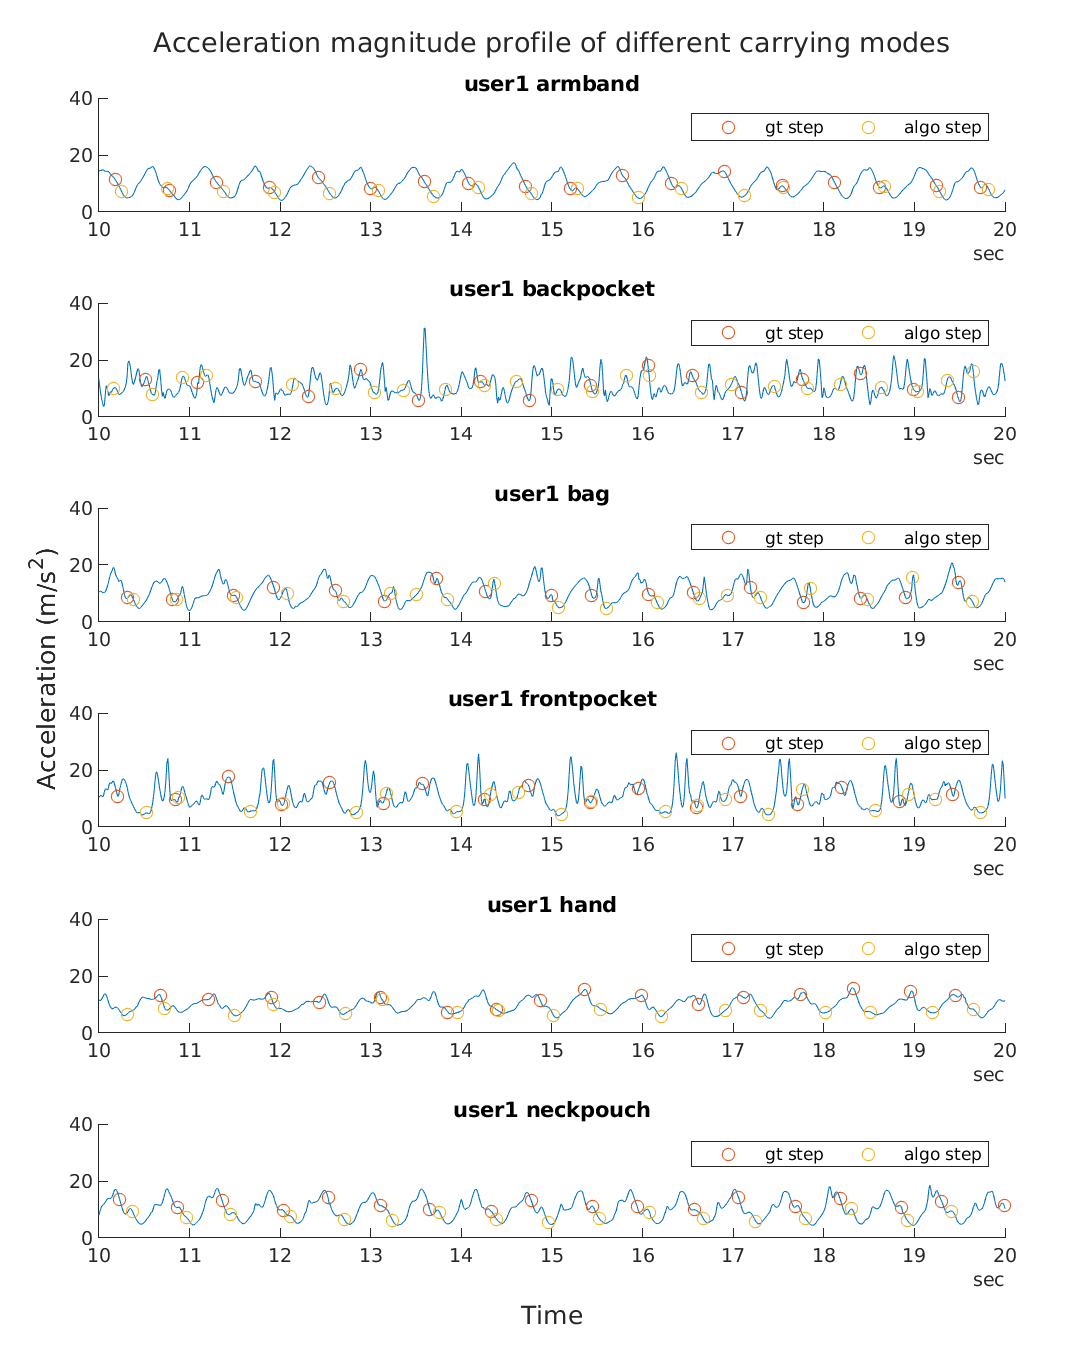
\includegraphics[width=\linewidth]{images/20200929_0951_gt_steps_vs_salvi_steps}
	\caption{extract of validation dataset from \citet{Salvi2018}, indicating ground truth steps and step detected by their algorithm.}
	\label{fig:gt_steps_vs_salvi_steps}
\end{figure}


The matlab algorithm, outlined in \cref{sec:meth - step detection}, could be applied on the validation data of the researchers. This allows it to be compared with a ground truth and with the solution of the researchers. \cref{fig:sd_comparison} shows how the matlab algorithm compares to the results in the validation datasets. \cref{fig:sd_abs_comparison} indicates the absolute number of steps detected. \cref{fig:sd_percent_comparison}  shows the percentage error compared to the ground truth, where  
positive percent error indicates over counting, while negative under counting. 
%TODO argument why it is different than what the research achieved.

\begin{figure}[H]
	\centering
	\begin{subfigure}[t]{.5\textwidth}
		\centering
		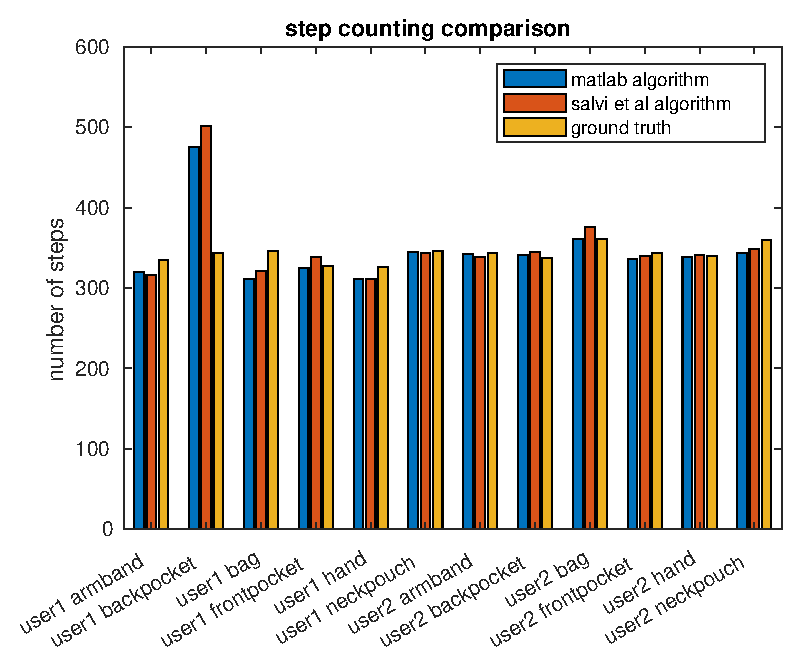
\includegraphics[width=\linewidth]{images/20200930_1214_step_counting_comparison}
		\caption{Absolute number of steps counted.}
		\label{fig:sd_abs_comparison}
	\end{subfigure}%
	\begin{subfigure}[t]{0.5\textwidth}
		\centering
		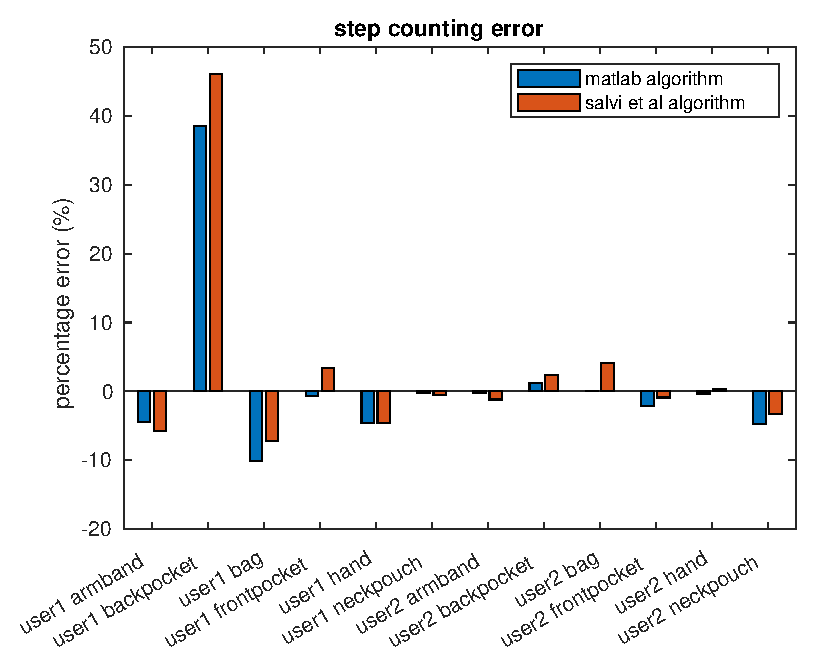
\includegraphics[width=\linewidth]{images/20200928_1248_step_counting_error}
		\caption{Percentage error from ground truth number of steps. }
		\label{fig:sd_percent_comparison}
	\end{subfigure}
	\caption{Comparison between \citet{Salvi2018} step detection algorithm, matlab algorithm and ground truth for different carrying modes.}
	\label{fig:sd_comparison}
\end{figure}

In addition to the data made available online, original data was gathered in which a subject walked exactly 60 steps while having a smartphone in 3 different carrying modes, backpocket, frontpocket and in hand. The percentage error from the ground truth can be seen in \cref{fig:202009291013step_counting_error_of_60_steps}.
\begin{figure}[H]
	\centering
	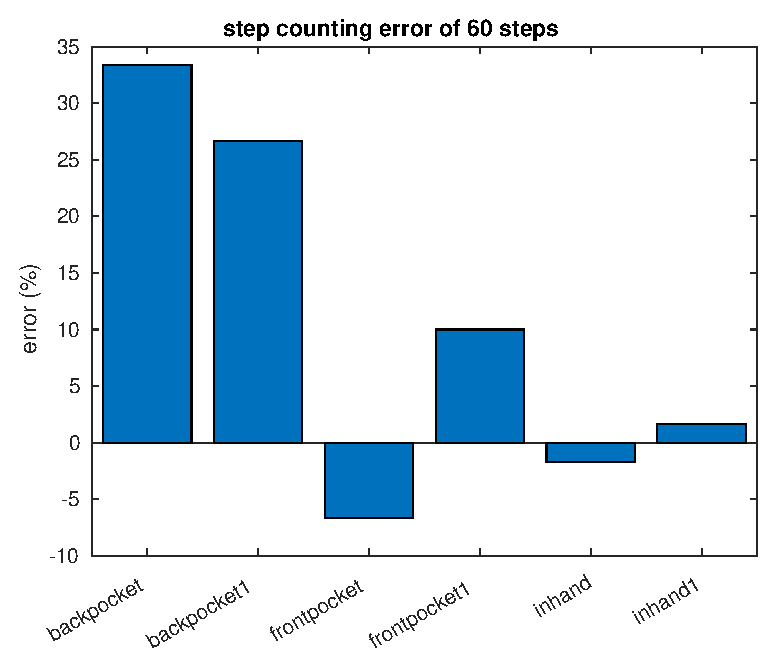
\includegraphics[width=0.6\linewidth]{images/20200929_1013_step_counting_error_of_60_steps}
	\caption{}
	\label{fig:202009291013step_counting_error_of_60_steps}
\end{figure}

For a PDR SHS it is not enough for the amount of steps to be accurate, but also the time when a step actually occurs. A step detection combined with the heading orientation at the moment of occurrence determines the vector in which the position estimate of the pedestrian will move. In order to ascertain how both the \citet{Salvi2018} algorithm and the algorithm from \cref{sec:meth - step detection} perform in this respect, true positive step detection was determined. Since it is unrealistic to expect the step detection to be at the exact time an actual step occurs, intervals are defined where if both a step occurs and is detected, the detection counts as a true positive. If in this interval two steps are detected, both detections are not considered true positive, and are considered a true positive double count. The time interval is increase itteratively in attempt to find the highest true positive count for both algorithms. The results can be found in \cref{fig:sd_tp_fp_comparison}
\begin{figure}[H]
	\centering
	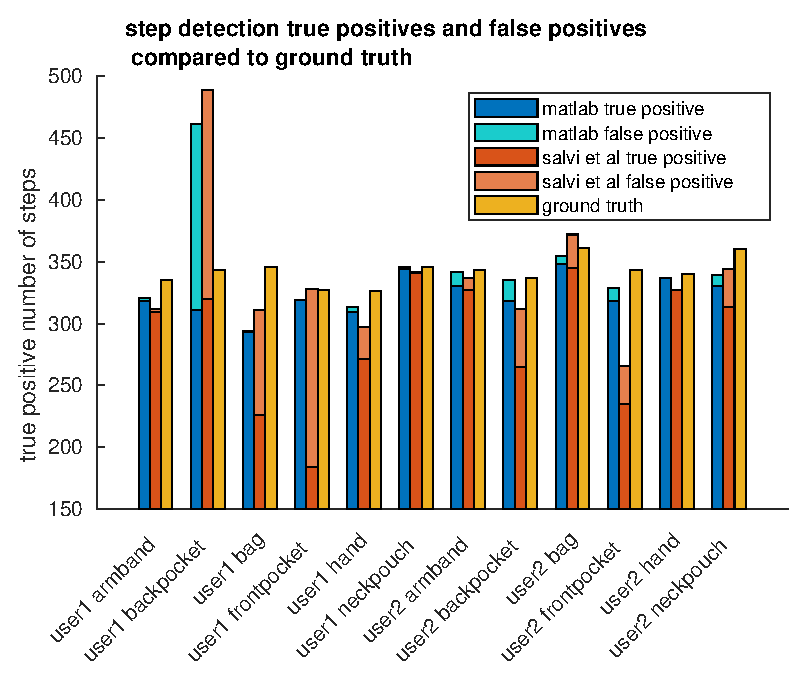
\includegraphics[width=0.7\linewidth]{images/20200930_1510_tp_fp_abs_comparison}
\caption{Comparison between \citet{Salvi2018} step detection algorithm, matlab algorithm and ground truth for different carrying modes.}
\label{fig:sd_tp_fp_comparison}
\end{figure}

\newpage

\section{Step Length Estimation}

\citet{Vezocnik2019} have also made the data they used open source. This data consist of accelerometer data of 15 different people for three walking speeds and in four smartphone carrying modes. Metrics for each test subject are collected, including height, gender and leg length. The walking modes were qualitative, in that they were either slow, normal, or fast walking speed. The carrying modes include the smartphone in pocket, in a bag, in the hand with the phone screen parallel to the floor, and in hand will swinging the carrying arm. Each person has two measurements for each combination, one for a 15 meter long straight path and another for 108 meter long straight path. The test subjects are not forced to walk these distances exactly, allowing for natural termination of their trial. \\
As done in \cite{Vezocnik2019} the smaller length set can be used to determine the parameter and the second to assess the performance.The best performing algorithm for global parameters is reiterated in \cref{eq:Tian2016_sle2} for convenience, where $h$ is the users height and $F$ is the step frequency. 

\begin{equation}
\label{eq:Tian2016_sle2}
\text{step size} = K \cdot h \cdot \sqrt{F}.
\end{equation}

In order to determine the tunable parameter $K$ correctly for the SHS, it needs to be used with the output of the step detection algorithm. This is because step detection will have a direct effect on the step frequency. The step detection algorithm cannot guarantee that all steps are counted, potentially affecting the tunable parameter. 
From the results of step detection, the most accurate results came from holding a smartphone in the hand. This carrying mode is present in the data from \cite{Vezocnik2019}, and can therefore be used for analysis. The results are shown in \cref{fig:step_length_estimation}. Here the parameters for \cref{eq:Tian2016_sle2} of all three walking speeds are plotted. In order to find $K$ as a universal constant a least square estimation is performed, shown by the green striped line in the plot.
\begin{figure}[H]
	\centering
	\begin{subfigure}[t]{.45\textwidth}
	\centering
	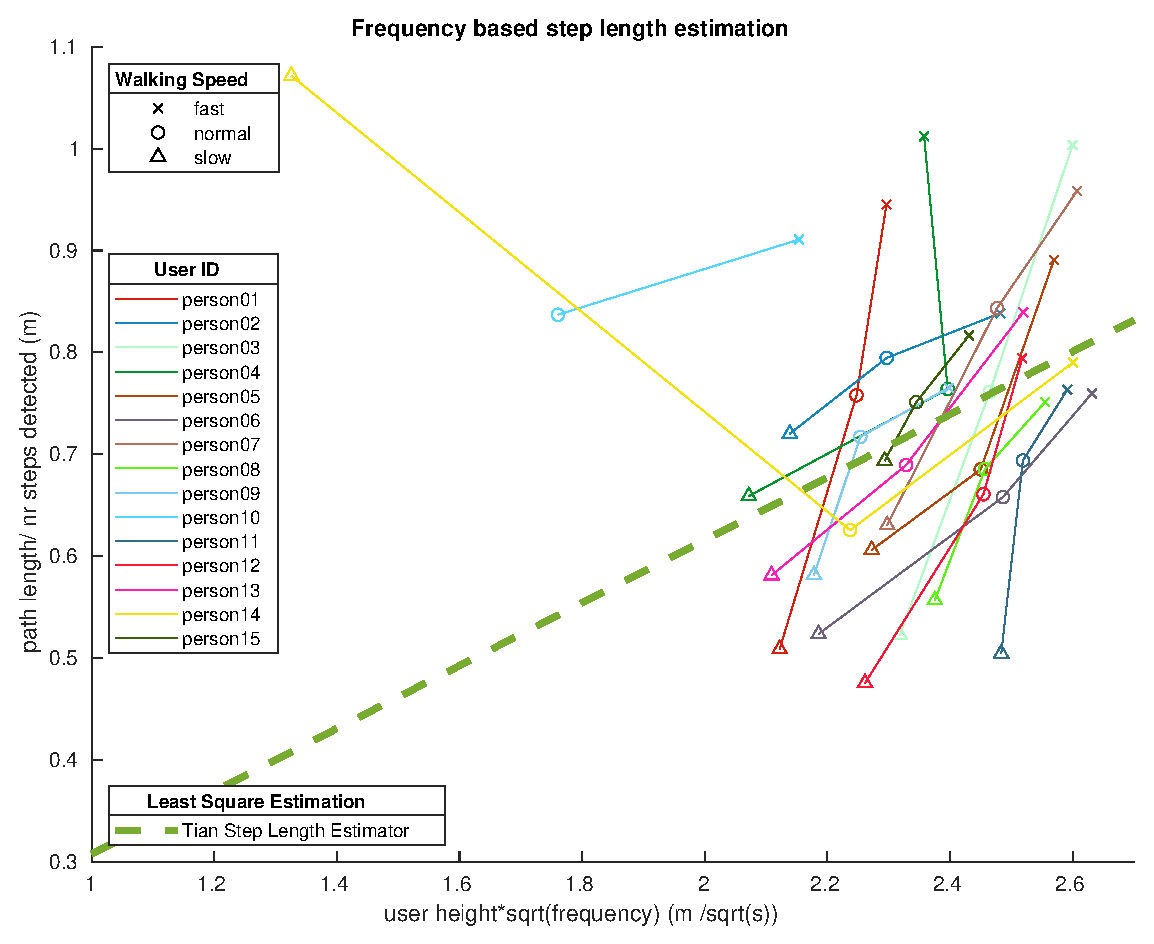
\includegraphics[width=\linewidth]{images/20201028_1050_step_length_all_data}
	\caption{step length estimation constant = 0.3116}
	\label{fig:step_length_all_data}
	\end{subfigure}
	\begin{subfigure}[t]{.45\textwidth}
		\centering
		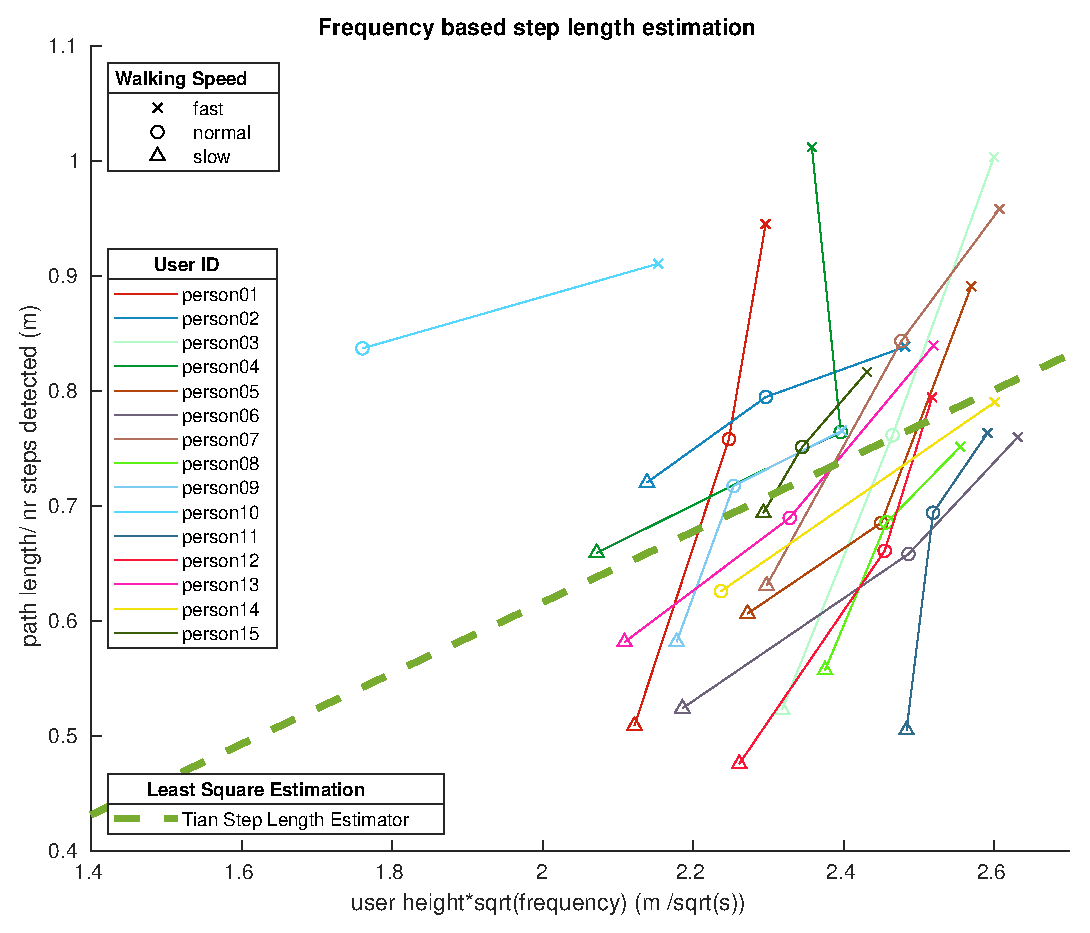
\includegraphics[width=0.95\linewidth]{images/20201028_1051_step_length_good_data}
		\caption{step length estimation constant = 0.3080}
		\label{fig:step_length_without_faults}
	\end{subfigure}
	\caption{step length estimation}
	\label{fig:step_length_estimation}
\end{figure}
Using the open source data has not come without problems, as can be seen in \cref{fig:step_length_all_data}. While most data seems to have relatively good step detection, there are two samples that do not conform to the general trend suggesting that step detection is not working correctly. The two potentially faulty data points are the slow walking sample of both person 10 and 14. For the former, no steps have been detected and is therefore not visible in the plots, while for the latter too little steps have been detected. For person 14, 14 steps have been detected for slow walking, which is less steps than when the subject was walking fast. This clearly suggests that a wrong step detection occurred. It is difficult to determine why this is occurring since the exact details. It could be that during this sample, the test subject was holding the phone incorrectly, the person had a very different step strategy when performing at this speed, or the phone was malfunctioning. This outlier affects the eventual tunable parameter. Removing it will change the estimate, as shown in \cref{fig:step_length_without_faults}. The performance of the step length estimate can be checked by using the validation dataset, where all users walked a longer distance, but with the same experimental setup. Here the accelerometer data can be passed through step detection and step length estimation to estimate the total distance traveled. This can then be compared with the actual distance traveled to determine the error. The data can also be used to determine if the difference in tunable parameter has a significant affect on the estimate. The results are found in  \cref{fig:step_length_estimation_validation}, where the absolute distance error for all walking speeds for all test subjects are shown, indicated by the dataset ID.
\begin{figure}[H]
	\centering
	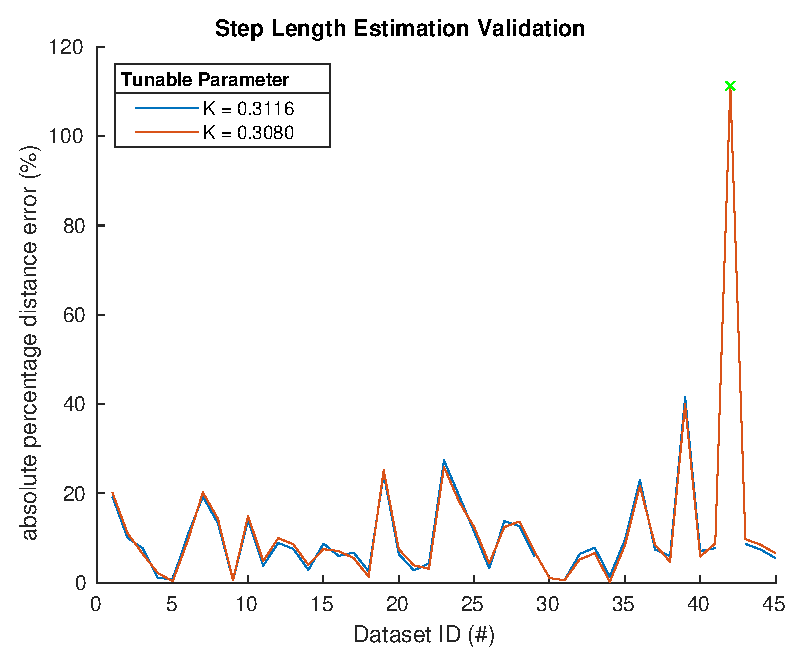
\includegraphics[width=0.6\linewidth]{images/20201028_1344_Step_Length_Estimation_Validation}
	\caption{}
	\label{fig:step_length_estimation_validation}
\end{figure}

What is noticeable from the results is that there is a large outlier. This is with dataset 42, which corresponds to the slow walking speed of test subject 14, which is also the setting in which the tunable parameter estimation had an outlier. This further supports that there is something significantly different when this test subject is performing at this walking speed. With this outlier the mean absolute error is 11.8 percent with a standard deviation of 17.1 percent. Without the outlier, the mean absolute error is 9.7 percent with a standard deviation of 8.0 percent. Both results are worse than those cited by \cite{Vezocnik2019}, which indicate a mean of 7 percent with a standard deviation of 5 percent.
The results also indicate that the different tunable parameters do not make a significant difference in accuracy. \par 
A similar smaller scale experiment was performed with three different people also walking at three different walking speeds. The results can be found in \cref{fig:step_length_personal_testing}. 
\begin{figure}[H]
	\centering
	\includegraphics[width=0.7\textwidth]{example-image-a}
	\caption{}
	\label{fig:step_length_personal_testing}
\end{figure}

{\color{red} still need to add comment on results }

\newpage

\section{Indoor Experiments}

Due to restriction caused by the COVID-19 pandemic, indoor testing was located at the house of a family member. The test consisted of walking around indoors with a smartphone in hand, and recording the IMU signals in the phone through an app, while also filming the path that is being walked. During the experiment a smartwatch was worn around of the not smartphone hand and used to open doors. This opening of doors was also recorded using the app running on the smartphone, which had a button to record timestamps. The full experimental process can be found in \cref{appendix:shs_experiment}. \par 
In order to use map information with the particle filter, different sources were combined to generate a map. Rudimentary paper blueprints of the building were available and could be photographed and traced in software to generate a picture of the indoor environment. This image has clear color distinction between the different structures within the building, including walls, doors and furniture. The positioning and size of furniture was estimated. The final image is seen in \cref{fig:indoor_blueprint}. This image is in pixel coordinates and needs to be transformed into meter coordinates. It then needs to represent a 2D probability density function so that it can be used in the particle filter measurement update. \\
The OccupancyMap in the MATLAB Robotics Tool box is suitable for this. An occupancy grid is a grid in which each cell has a value representing the probability of the occupancy of that cell. By measuring a known structure in Google Maps using the measurement tool and comparing with its pixel length in the image, a meter to pixel ratio can be defined. The Google Maps measurement can be found in \cref{fig:house_google_maps}. This pixel to meter ratio combined with the image, allows MATLAB to generate an occupancy grid as shown in \cref{fig:pf_map}. This same process can be used to get the meter position of all doors.

\begin{figure}[H]
	\centering
	\begin{subfigure}[t]{.3\textwidth}
	\centering
	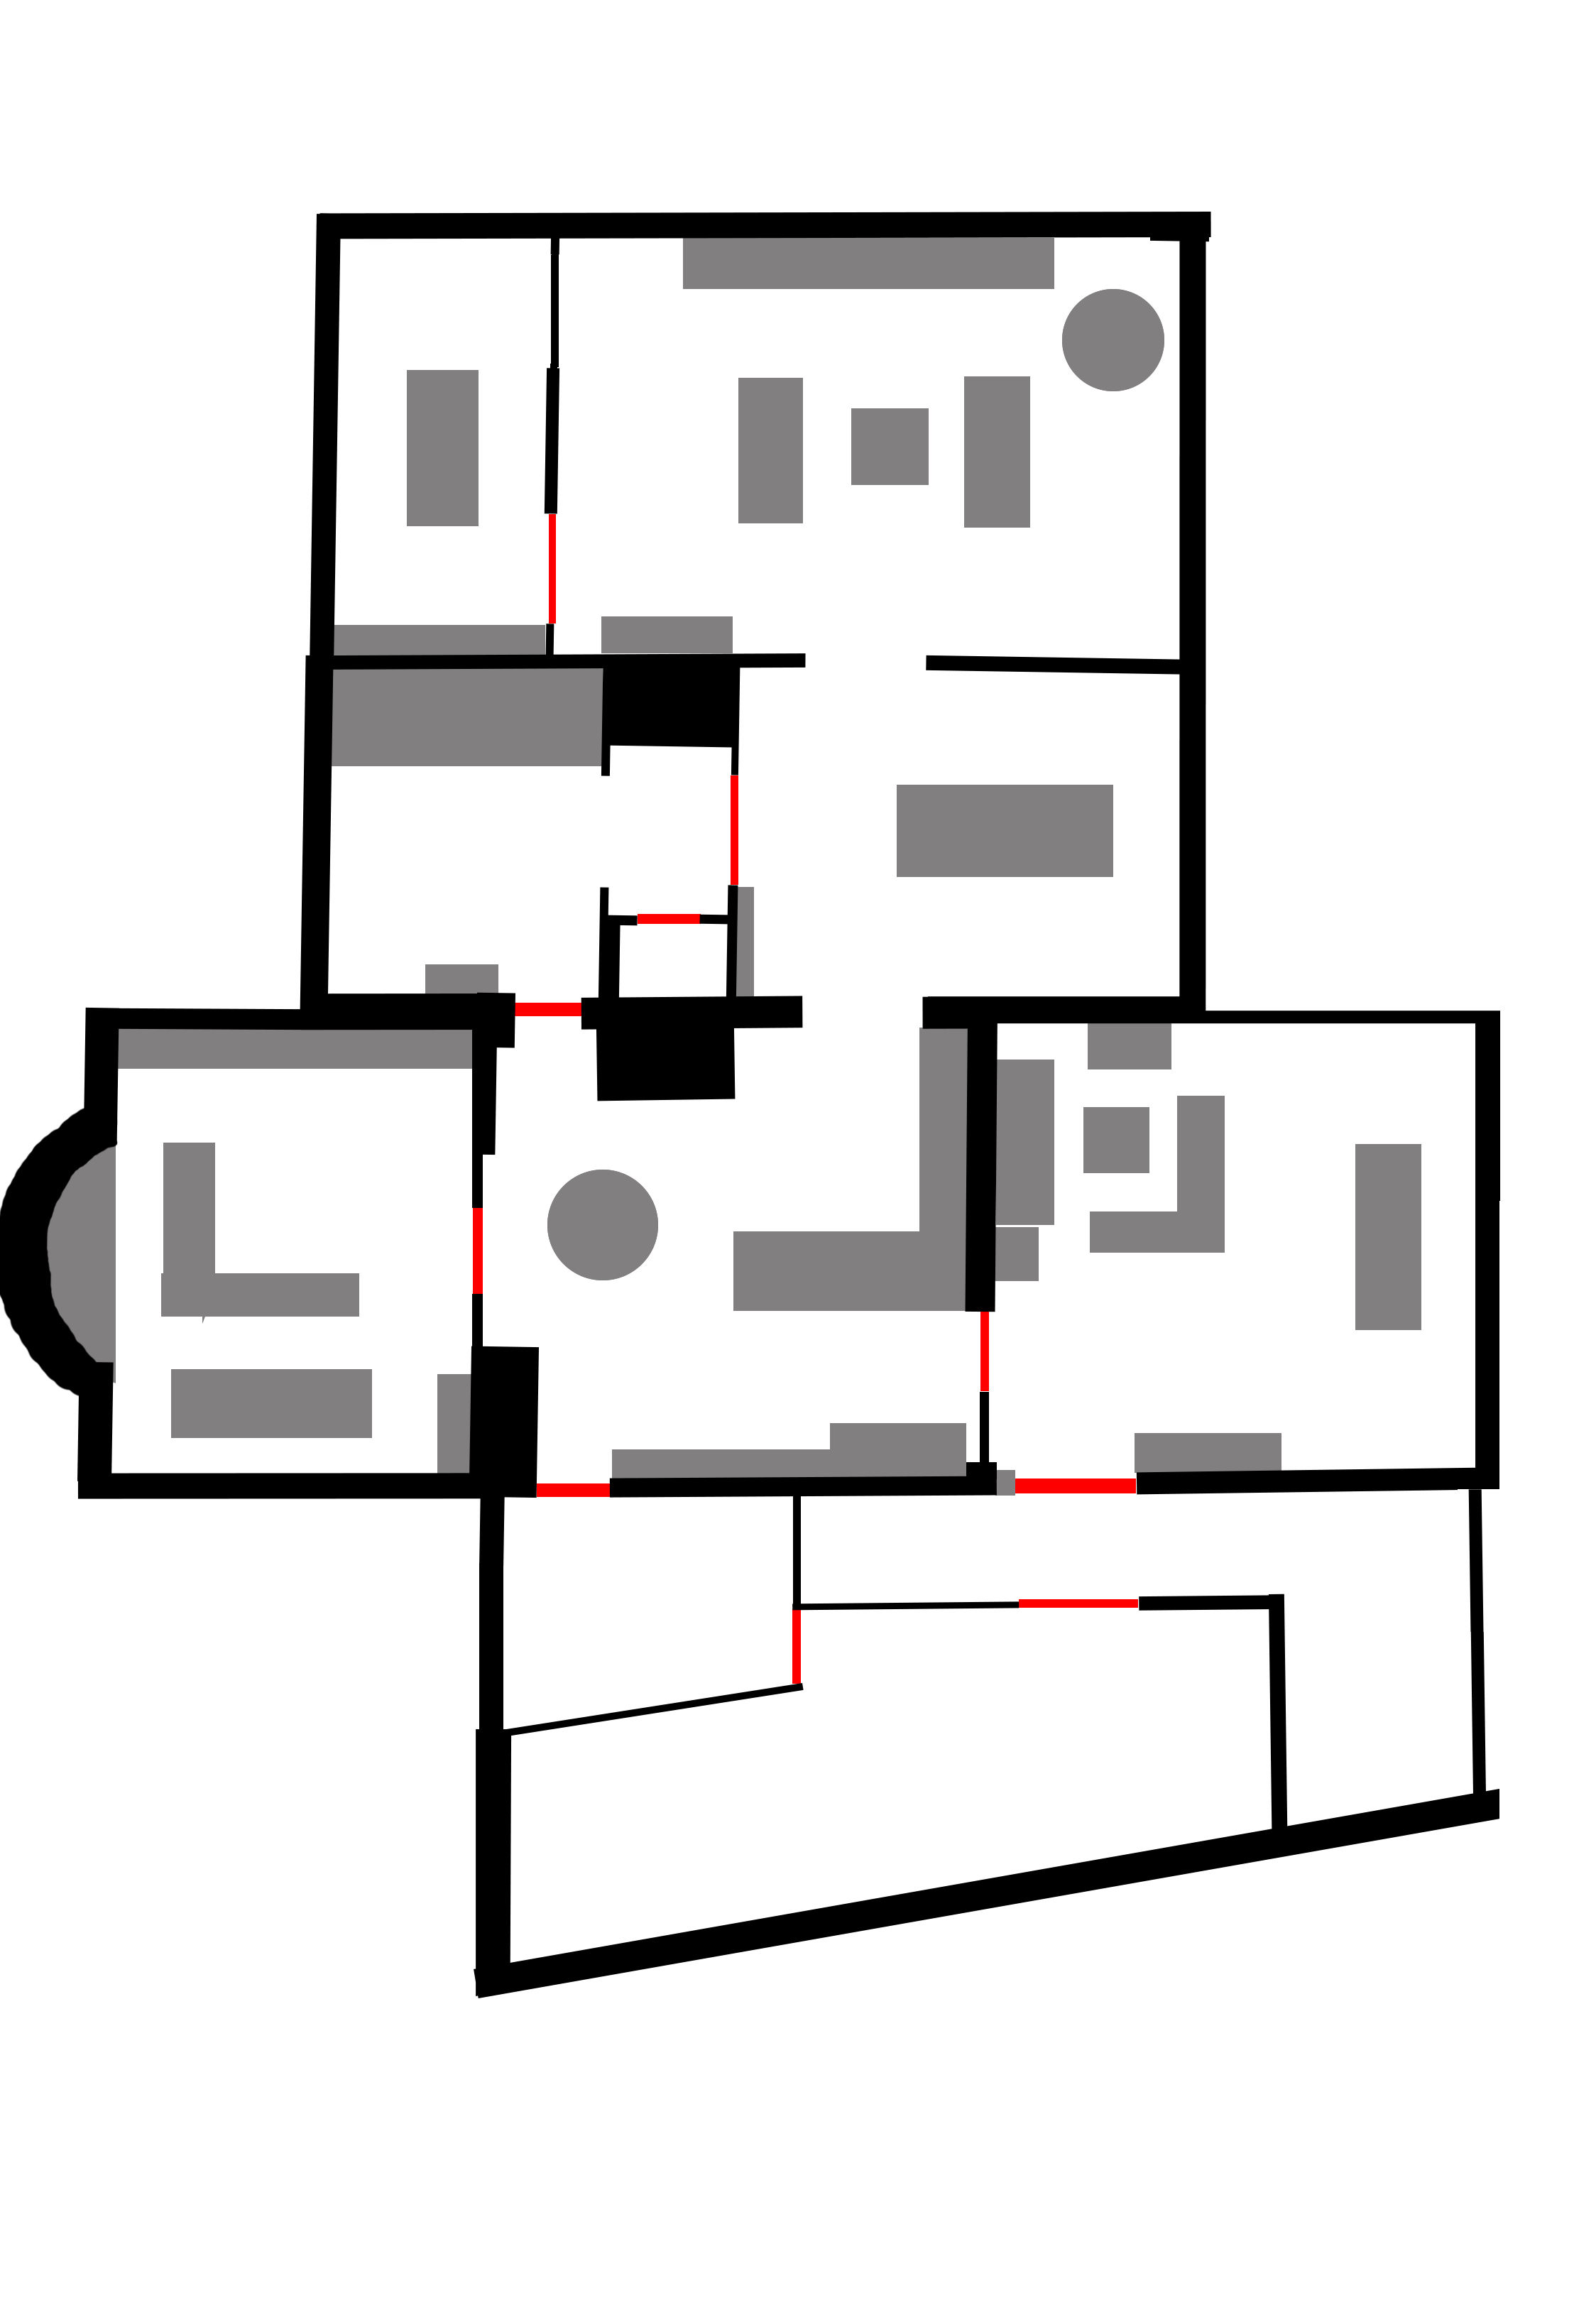
\includegraphics[width=0.9\linewidth]{images/indoor_blueprint}
	\caption[Image from building blueprints]{Image from building blueprints. Black, grey and red represent walls, furniture, and doors, respectively.}
	\label{fig:indoor_blueprint}
\end{subfigure} \quad
\begin{subfigure}[t]{.3\textwidth}
	\centering
	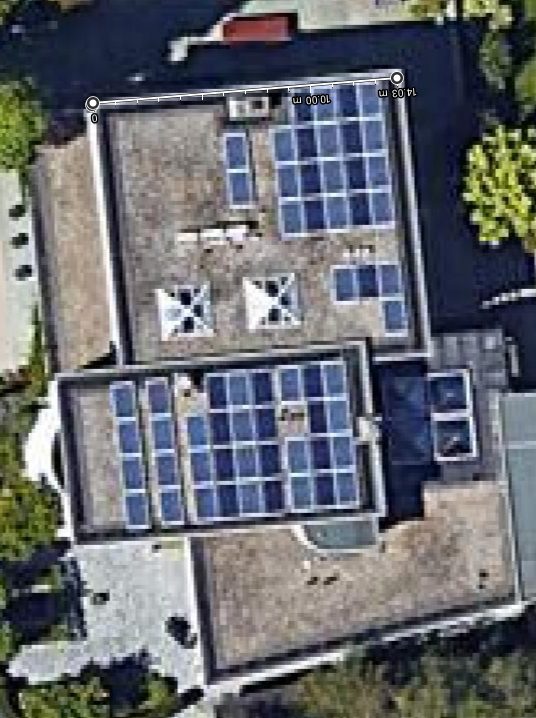
\includegraphics[width=0.9\linewidth]{images/house_google_maps}
	\caption{Measurement from Google Maps}
	\label{fig:house_google_maps}
\end{subfigure} \quad
\begin{subfigure}[t]{.3\textwidth}
	\centering
	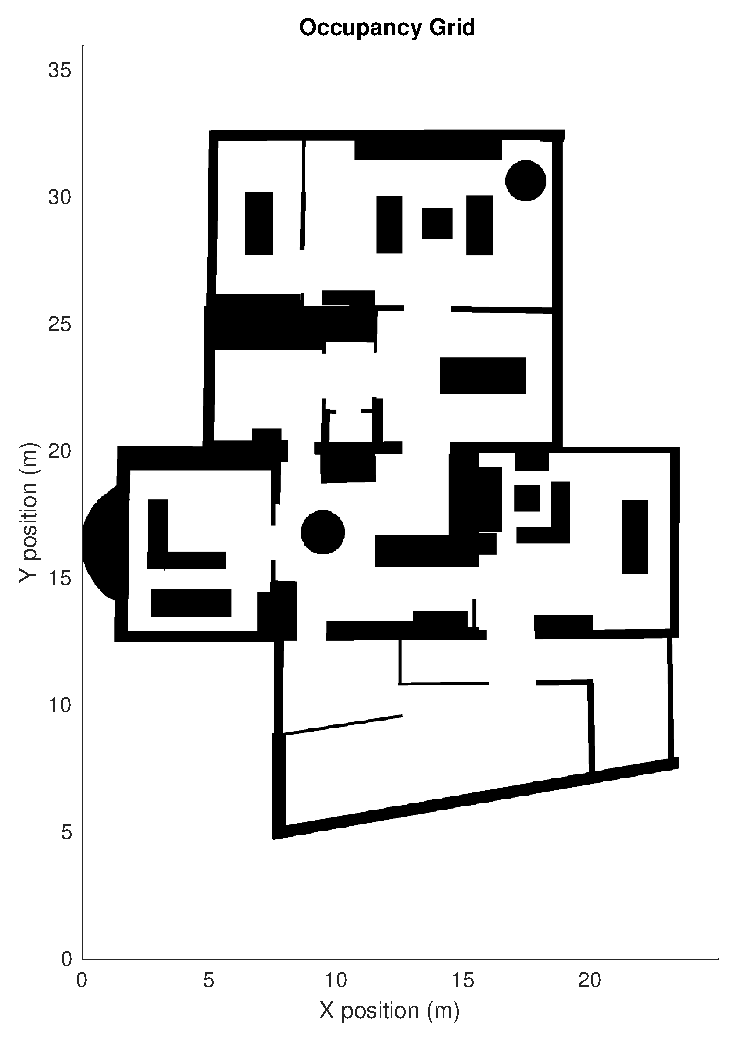
\includegraphics[width=0.9\linewidth]{images/20201030_1157_pf_map_1}
	\caption{Particle Filter map result}
	\label{fig:pf_map}
\end{subfigure}
\label{fig:particle_map_construction}
\caption{particle filter map creation}
\end{figure}

During the experiment, a total of 8 trials were walked by one test subject, each trying to generate a different trajectory than the previous trials. The video recorded during the experiment can be used in postprocessing to get a ground truth. This was done by replaying the video and at set intervals manually indicating approximately where on the map the test subject was located. The position and time elapsed were recorded. The output of these trials can be used to test certain SHS components individually and the system as a whole.



\subsection{Indoor Orientation Estimation}
The indoor orientation estimation method outlined in \cref{sec:method-EKF} can be compared with the output of the android operating system. Two examples can be found in 

\begin{figure}[H]
	\centering
	\begin{subfigure}[t]{.45\textwidth}
	\centering
	\includegraphics[width=0.7\textwidth]{example-image-a}
	\caption{Orientation estimation of trial 1 compared to android orientation estimation}
	\label{fig:trail1 - shs}
\end{subfigure}\quad
\begin{subfigure}[t]{.45\textwidth}
	\centering
	\includegraphics[width=0.7\textwidth]{example-image-b}
	\caption{Orientation estimation of trial 2 compared to android orientation estimation}
	\label{fig:trail2 - shs}
\end{subfigure}
\end{figure}

The error between each trial can be found in \cref{fig:orientation_comparison}.

\begin{figure}[H]
	\centering
	\includegraphics[width=0.7\textwidth]{example-image-c}
	\caption{}
	\label{fig:orientation_comparison}
\end{figure}

From these results it is shown that the error between my own orientation estimation and that calculated by the android system has similar performance.

\subsection{Step and Heading System}
All components of the step and heading system have been tested separately, giving an indication of their strengths and limitations. Now the whole system can be combined and tested in an indoor environment to evaluate the whole system performance. The output of the step and heading system will be the relative position change from a start point, known as dead reckoning.
For every trial the smartphone imu data is passed through the different components of the SHS outlined in this report. Each trajectory can then be compared to the ground truth generate through post processing as outlined at the beginning of this sections. Two trials with their trajectory projected onto the map and side by side comparison with the ground truth can be found in \cref{fig:trial1_shs_gt_comparison} and \cref{fig:trial2_shs_gt_comparison}. Note that the shs trajectories in these images have been rotated heuristically in order to fit the map as best as possible. This needs to be done since there is no way for the step and heading system output to know how to orient itself with respect to the building. This is because it does not have pre-existing knowledge on the orientation of the magnetic field inside the building.

\begin{figure}[H]
	\centering
	\begin{subfigure}[t]{.45\textwidth}
		\centering
		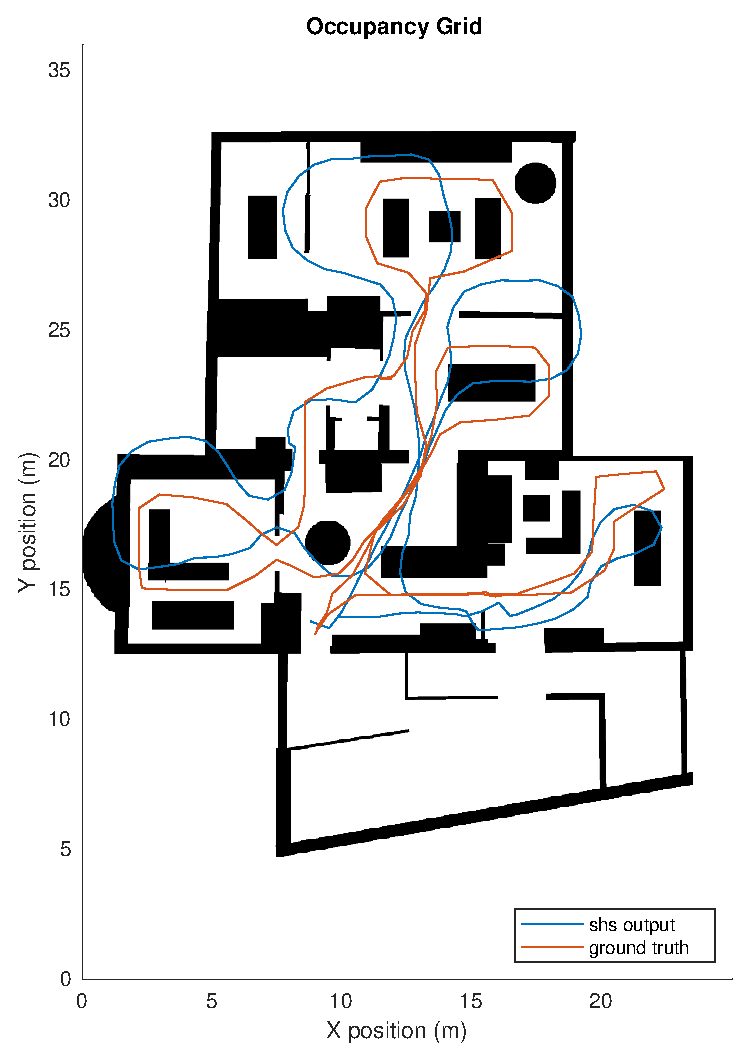
\includegraphics[width=0.9\linewidth]{images/20201029_1040_trial1_shs_1}
		\caption{trajectory comparison}
		\label{fig:trial1_on_map}
	\end{subfigure}
	\begin{subfigure}[t]{.45\textwidth}
		\centering
		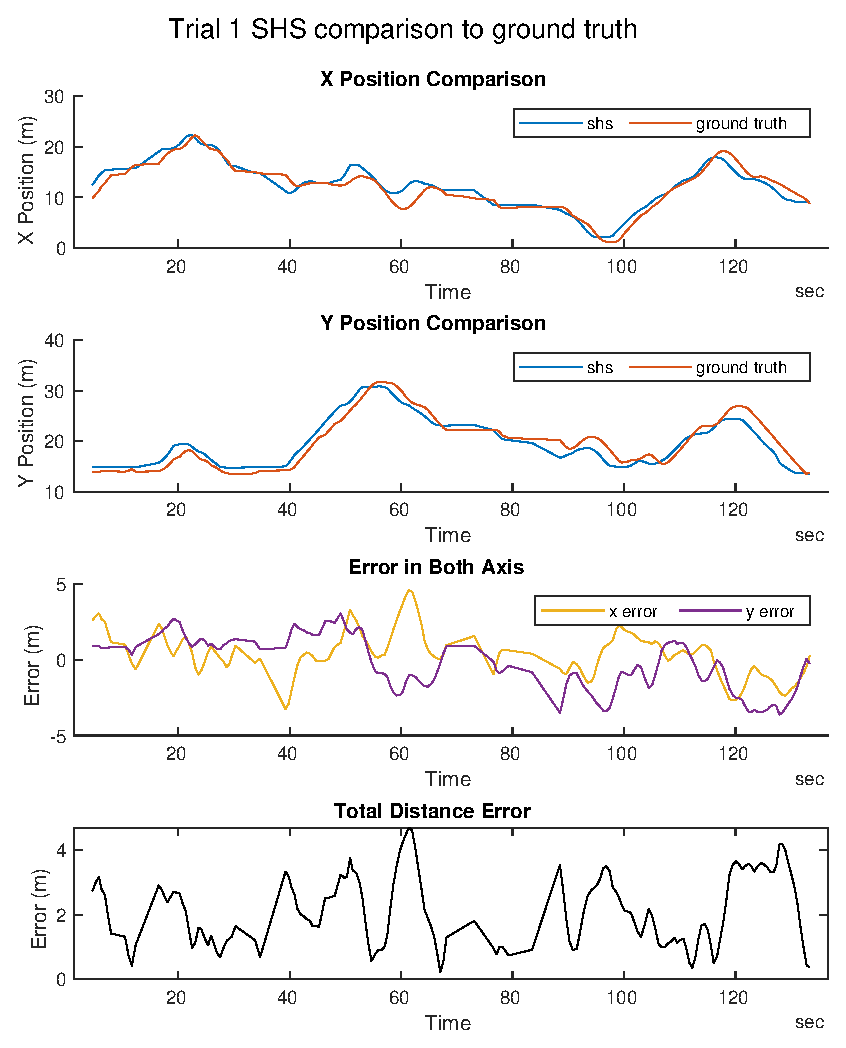
\includegraphics[width=\linewidth]{images/20201029_1040_trial1_shs_2}
		\caption{axis comparison}
		\label{fig:trial1_comparison}
	\end{subfigure}
	\caption{SHS comparison of trial 1 with ground truth}
	\label{fig:trial1_shs_gt_comparison}
\end{figure}

\begin{figure}[H]
	\centering
	\begin{subfigure}[t]{.45\textwidth}
		\centering
		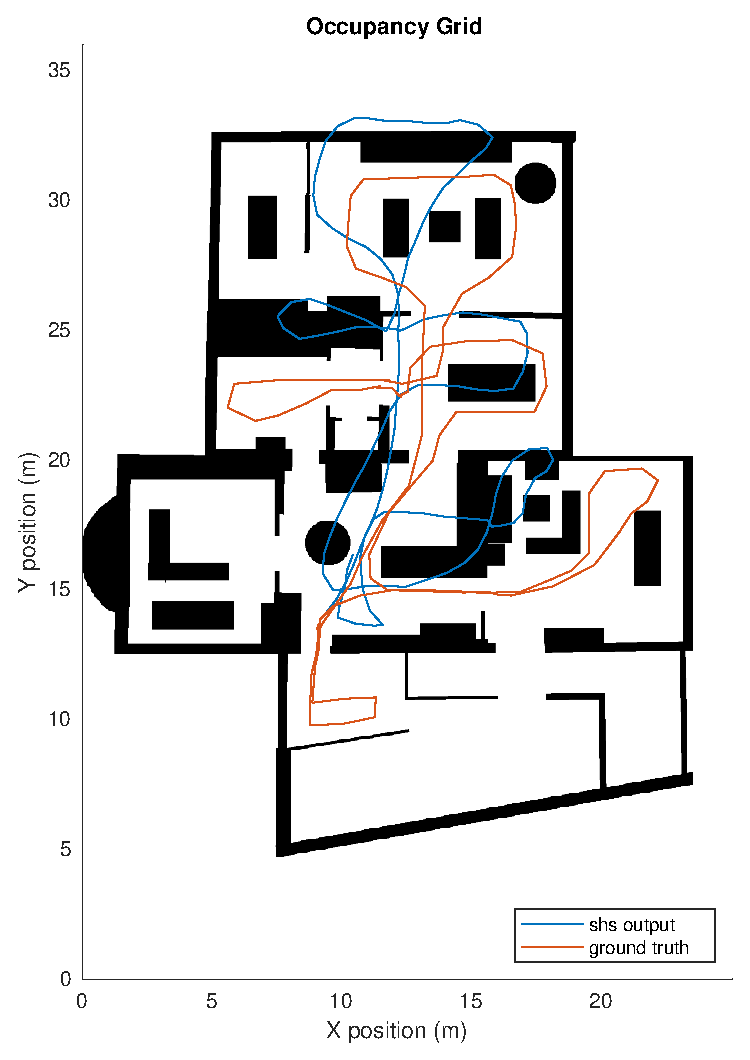
\includegraphics[width=0.9\linewidth]{images/20201029_1042_trial2_shs_1}
		\caption{trajectory comparison}
		\label{fig:trial2_on_map}
	\end{subfigure}
	\begin{subfigure}[t]{.45\textwidth}
		\centering
		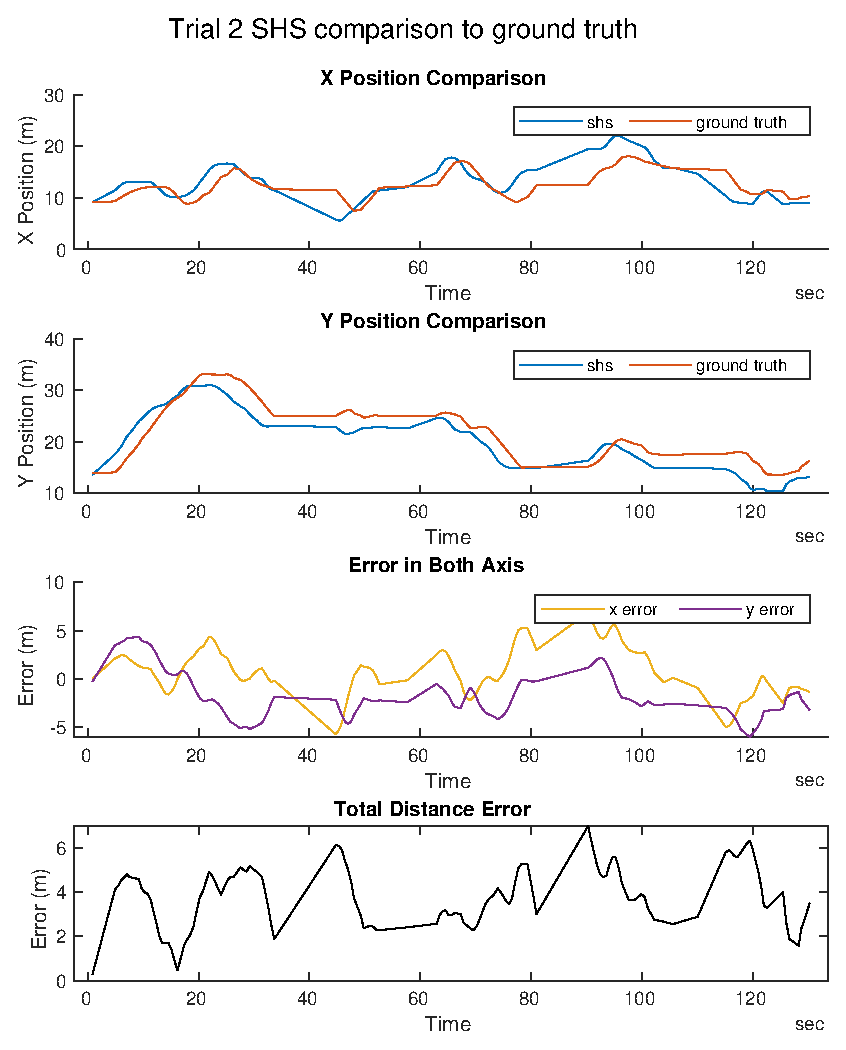
\includegraphics[width=\linewidth]{images/20201029_1042_trial2_shs_2}
		\caption{axis comparison}
		\label{fig:trial2_comparison}
	\end{subfigure}
	\caption{SHS comparison of trial 2 with ground truth}
	\label{fig:trial2_shs_gt_comparison}
\end{figure}


\subsection{Particle Filter}
Using the output of the SHS and the method outlined in \cref{sec:method-pf} for the particle filter, the indoor localization particle filter could be constructed 

\subsubsection{With activity }

\begin{figure}[H]
	\centering
	\begin{subfigure}[t]{.45\textwidth}
		\centering
		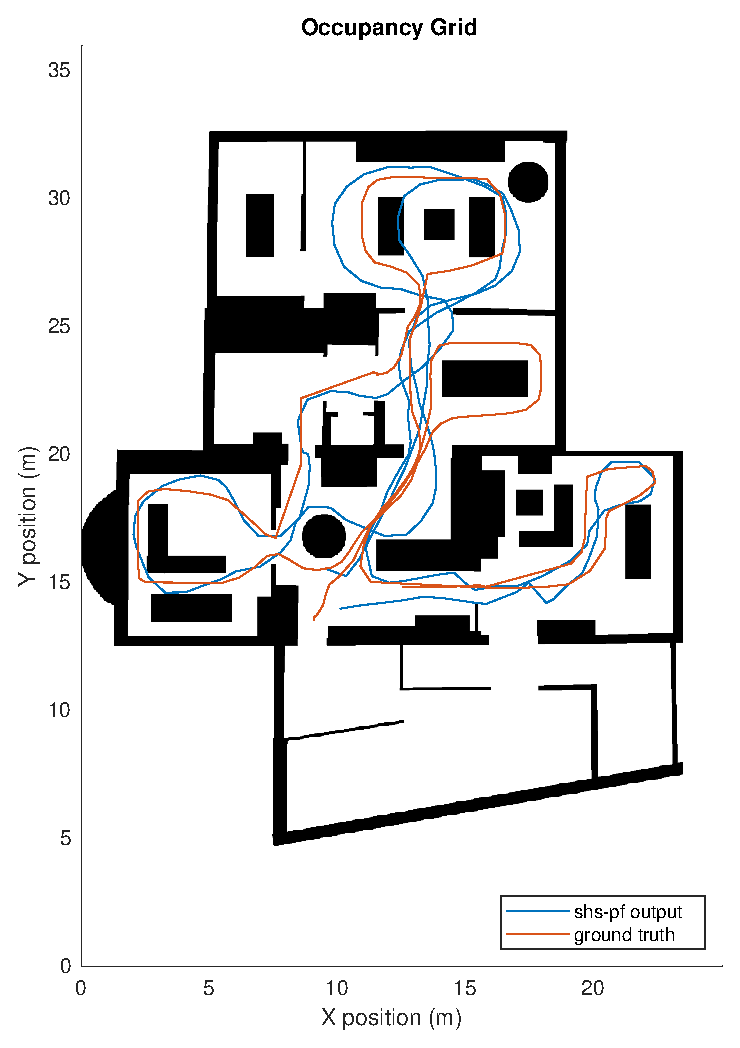
\includegraphics[width=0.9\linewidth]{images/20201029_1603_shs-pf_trial_1_2}
		\caption{trajectory comparison}
		\label{fig:shspf_trial2_on_map}
	\end{subfigure}
	\begin{subfigure}[t]{.45\textwidth}
		\centering
		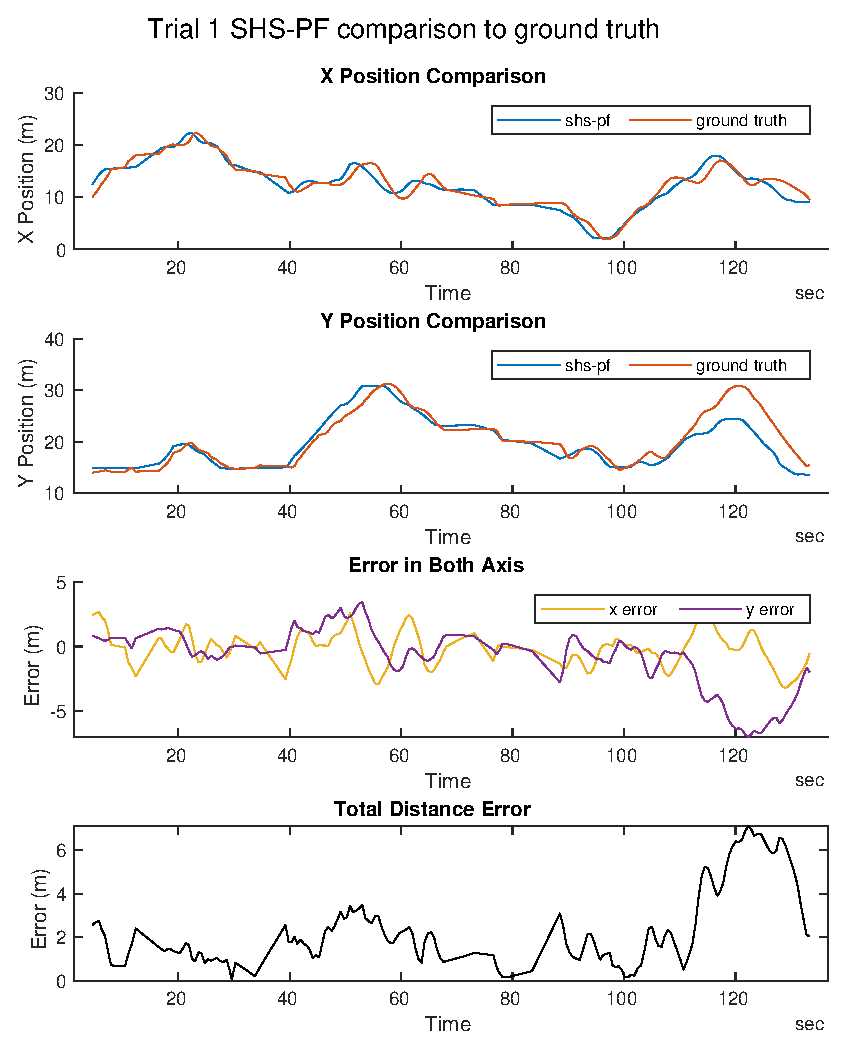
\includegraphics[width=\linewidth]{images/20201029_1603_shs-pf_trial_1_1}
		\caption{axis comparison}
		\label{fig:shspf_trial2_comparison}
	\end{subfigure}
	\caption{SHS comparison of trial 2 with ground truth}
	\label{fig:shspf_trial2_shs_gt_comparison}
\end{figure}

\begin{figure}[H]
	\centering
	\begin{subfigure}[t]{.45\textwidth}
		\centering
		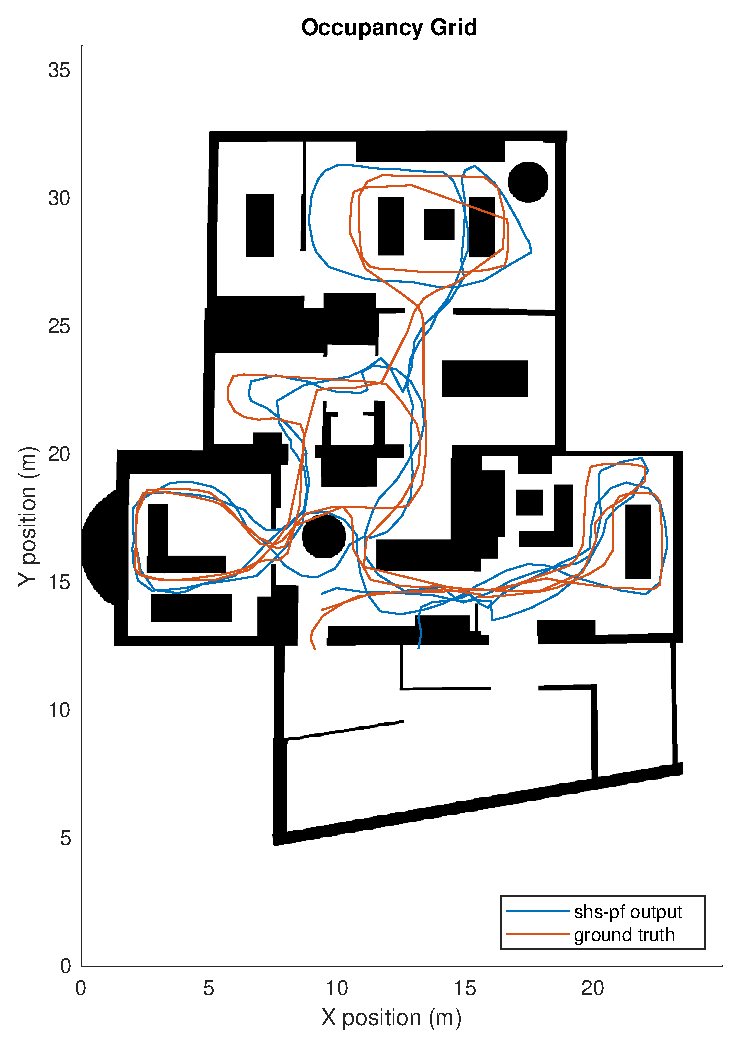
\includegraphics[width=0.9\linewidth]{images/20201029_1804_shs-pf_trial_3_2}
		\caption{trajectory comparison}
		\label{fig:shspf_trial3_on_map}
	\end{subfigure}
	\begin{subfigure}[t]{.45\textwidth}
		\centering
		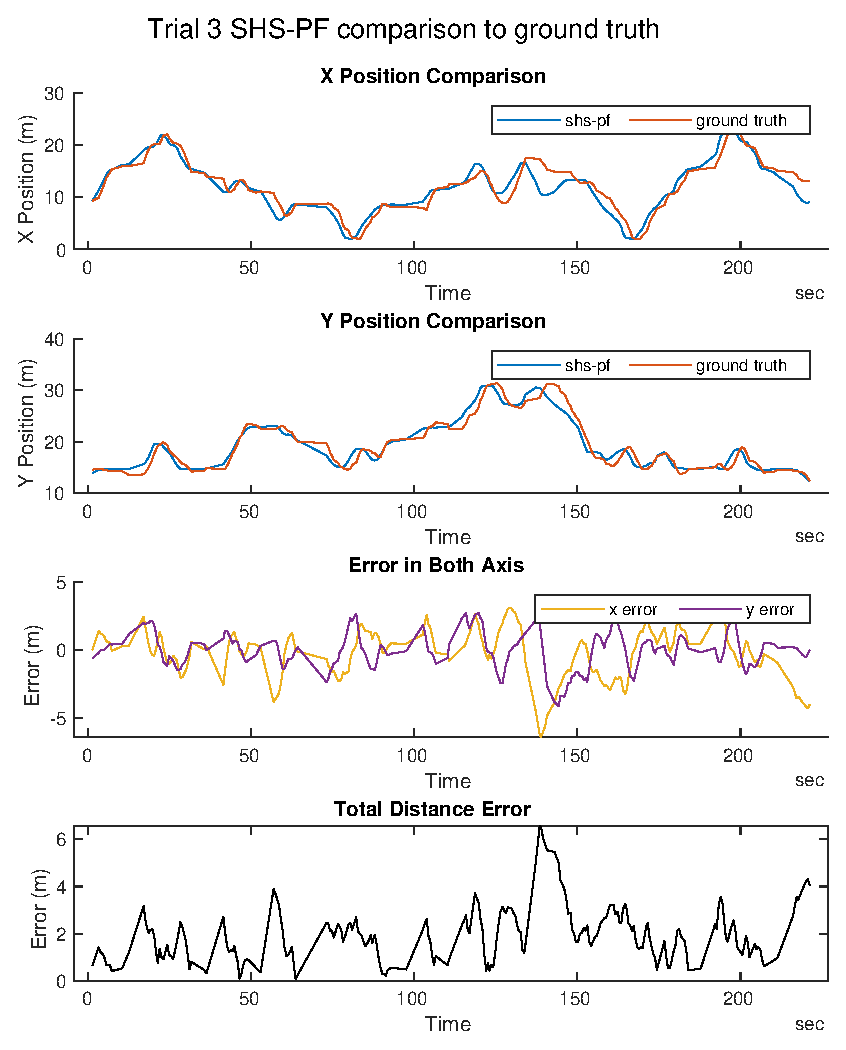
\includegraphics[width=\linewidth]{images/20201029_1804_shs-pf_trial_3_1}
		\caption{axis comparison}
		\label{fig:shspf_trial3_comparison}
	\end{subfigure}
	\caption{SHS comparison of trial 5 with ground truth}
	\label{fig:shspf_trial3_shs_gt_comparison}
\end{figure}

\section{Activity Recognition}
